\section{Patterns 6 - Redegør for følgende concurrency mønstre}

\subsection{Fokuspunkter}

\begin{itemize}
	\item Parallel Aggregation.
	\item MapReduce.
\end{itemize}

\subsection{Parallel Aggregation}
I forlængelse af parallelle loop kan det sige at ikke alle PL's iterationer eksekveres uafhængigt. Fx et loop der udregner en sum, bruger hver iterations resultat til at akkumulere en enkelt variabel der indeholder den udregnede sum op til det iterationsniveua vi er på. Denne akkumulerede værdi er en aggregation.\\

Man Skulle dermed tro at at aggregation operation ikke kan forenees med PL. Dog findes der en vej! Parallell aggregation pattern!\\

Dette pattern benytter \textit{unshared} lokale variabler som merges til slut for at give det endelige resultat. PA kaldes også parallel reduction pattern, idet den kombinerer flere inputs til et enkelt output.

Tag eksempelvis udtrykket \textit{a + b + c + d}. Istedet for at løse dette sekventielt:

\textit{((a + b) + c) +d}

Kan vi sige:

\textit{(a + b) + (c + d)}

Den sidste metode kan vi løse parallelt. Og det er dette der er meningen med Parallel Aggregation.

Illustreret har vi:

\begin{figure}[H]
	\centering
	\begin{minipage}{.4\textwidth}
		\centering
		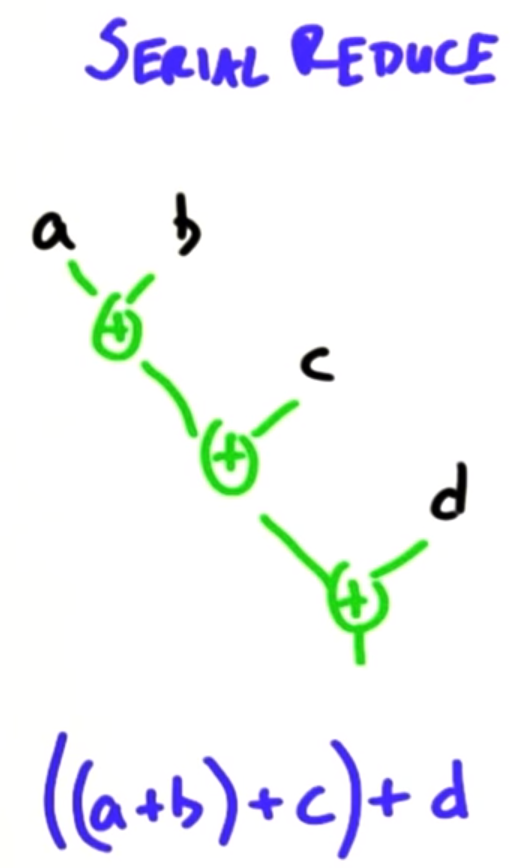
\includegraphics[width=0.8\linewidth]{figs/aggregation/seqReduce}
		\captionof{figure}{Sekventiel reducering}
		\label{seqReduce}
	\end{minipage}
	\begin{minipage}{.4\textwidth}
		\centering
		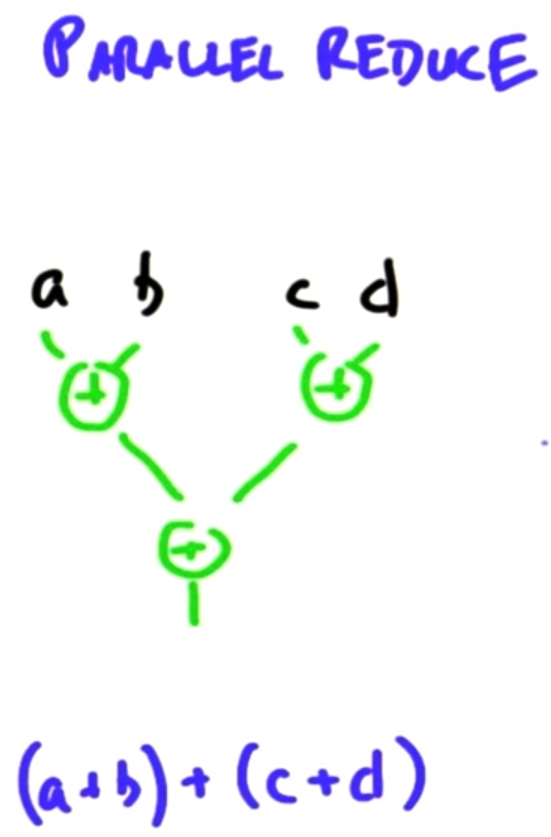
\includegraphics[width=0.8\linewidth]{figs/aggregation/paraReduce}
		\captionof{figure}{Parallel reducering}
		\label{paraReduce}
	\end{minipage}
\end{figure}

\subsection{MapReduce}
MapReduce er en måde at arbejde på meget store datasæt. Der arbejdes med MapReduce parallelt på dataen.

\subsubsection{4 steps}
Vi kan opdele MapReduce modellen i 4 steps:\\

Eksempel med spillekort:

Vi ønsker at vide hvor mange af hver kulør der findes i vores stak.
\begin{enumerate}
	\item \textbf{Distribuer source data til forskellige nodes.}\\
	Fordel stakken af kort ud på alle noder.
	\item \textbf{Map data - Repræsenter data i key-value par.}\\
	Hver node tæller hvor mange af hver kulør den har fået tildelt. Dette repræsenteres med key-value par. eg. Kulør (key) og kortværdi (value).
	\item \textbf{Gruppér data.} \\
	Grouperen har til ansvar at gruppere mappernes key-value par. Her tages alle klør par og sættes i samme gruppe, alle ruder par sættes sammen osv.
	\item \textbf{Reducer eller merge  data fra grouperen.}\\
	Her tælles sammen hvor mange af hver kulør der er i de grupperede data.
\end{enumerate}
